\documentclass[utf8]{beamer}

\mode<presentation>
{
  \usetheme{Warsaw}
  \setbeamercovered{transparent}
}


\usepackage{amsfonts,mathtools,amssymb}
\usepackage[spanish]{babel}
\usepackage{times}
\usepackage[T1]{fontenc}
\usepackage[shortlabels]{enumitem}
\usepackage{tikz}
\usepackage{physics}

\title[MA0505]{MA0505 - An\'alisis I}
\subtitle{Lecci\'on XIII: La Medida de Lebesgue II}

\author{Pedro M\'endez\inst{1}}

\institute[Universidad de Costa Rica] % (optional, but mostly needed)
{
  \inst{1}%
  Departmento de Matem\'atica Pura y Ciencias Actuariales\\
  Universidad de Costa Rica
  }

\date[I-2021] {Semestre I, 2021}

%%%%%%%%% === Theorems and suchlike === %%%%%%%%%%%%%%

\theoremstyle{plain}
\newtheorem{Th}{Teorema}               %%% Theorem 1.1.1
\newtheorem{Tmon}{Teoremón}
\newtheorem{Prop}{Proposición}         %%% Proposition 1.1.2
\newtheorem{Lem}{Lema}                 %%% Lemma 3
\newtheorem{Cor}{Corolario}            %%% Corollary 4

\theoremstyle{definition}
\newtheorem{Def}{Definición}           %%% Definition 5
\newtheorem{Ex}{Ejemplo}               %%% Example 6
\newtheorem{Ej}{Ejercicio}             %%% Ejercicio 7
\newtheorem{Hec}[Th]{Hecho}            %%% Hecho 1.1.8

\theoremstyle{remark}
\newtheorem{Rmk}[Th]{Observación}      %%%Remark 1.1.9
\newtheorem*{nonum-Rmk}{Observación}         %%% No number Fact
\newtheorem*{Notn}{Notaci\'on}        %% Notaciones
\newtheorem*{Warn}{Advertencia}       %% Advertencias

\numberwithin{equation}{section}

%% Accomodations 

\makeatletter
\def\moverlay{\mathpalette\mov@rlay}
\def\mov@rlay#1#2{\leavevmode\vtop{%
   \baselineskip\z@skip \lineskiplimit-\maxdimen
   \ialign{\hfil$\m@th#1##$\hfil\cr#2\crcr}}}
\newcommand{\charfusion}[3][\mathord]{
    #1{\ifx#1\mathop\vphantom{#2}\fi
        \mathpalette\mov@rlay{#2\cr#3}
      }
    \ifx#1\mathop\expandafter\displaylimits\fi}
\makeatother

% Greek letters:

\newcommand{\al}{\alpha}                %% short for  \alpha
\newcommand{\bt}{\beta}                 %% short for  \beta
\newcommand{\Dl}{\Delta}                %% short for  \Delta
\newcommand{\dl}{\delta}                %% short for  \delta
\newcommand{\eps}{\varepsilon}          %% short for  \varepsilon
\newcommand{\Ga}{\Gamma}                %% short for  \Gamma
\newcommand{\ga}{\gamma}                %% short for  \gamma
\newcommand{\La}{\Lambda}               %% short for  \Lambda
\newcommand{\la}{\lambda}               %% short for  \lambda
\newcommand{\Om}{\Omega}                %% short for  \Omega
\newcommand{\om}{\omega}                %% short for  \omega
\newcommand{\Sg}{\Sigma}                %% short for  \Sigma
\newcommand{\sg}{\sigma}                %% short for  \sigma
\newcommand{\te}{\theta}                %% short for  \theta
\newcommand{\vf}{\varphi}               %% short for  \varphi
\newcommand{\ze}{\zeta}                 %% short for  \zeta

%Boldface letters

\newcommand{\bC}{\mathbb{C}}    %%% números complejos
\newcommand{\bN}{\mathbb{N}}    %%% números naturales
\newcommand{\bP}{\mathbb{P}}        %% números enteros positivos
\newcommand{\bQ}{\mathbb{Q}}    %%% números racionales
\newcommand{\bR}{\mathbb{R}}    %%% números reales
\newcommand{\bS}{\mathbb{S}}    %%% esfera
\newcommand{\bZ}{\mathbb{Z}}    %%% números enteros

%Script letters:

\newcommand{\cA}{\mathcal{A}}           %% formas diferenciales
\newcommand{\cB}{\mathcal{B}}           %% una base vectorial
\newcommand{\cC}{\mathcal{C}}           %% otra base vectorial
\newcommand{\cF}{\mathcal{F}}           %% espacio de Fock
\newcommand{\cL}{\mathcal{L}}           %% operadores lineales
\newcommand{\cM}{\mathcal{M}}           %% multiplicadores
\newcommand{\cN}{\mathcal{N}}           %% funciones nulas
\newcommand{\cP}{\mathcal{P}}           %% una particion
\newcommand{\cR}{\mathcal{R}}           %% funciones representativas
\newcommand{\cS}{\mathcal{S}}           %% funciones de Schwartz


%Brackets

\newcommand{\bonj}[1]{\left\lbrack#1\right\rbrack}
\newcommand{\obonj}[1]{\left\rbrack#1\right\lbrack}
\newcommand{\rbonj}[1]{\left\rbrack#1\right\rbrack}
\newcommand{\lbonj}[1]{\left\lbrack#1\right\lbrack}
\newcommand{\snm}[1]{\|#1\|}           %small norma
\newcommand{\nm}[1]{\left\|#1\right\|} %norma pegadita
\newcommand{\pnm}[1]{\biggl|\biggl|#1\biggr|\biggr|}
\newcommand{\set}[1]{\{\,#1\,\}}    %% set notation
\newcommand{\floor}[1]{\lfloor#1\rfloor} %% mayor entero <= x
\newcommand{\Set}[1]{\biggl\{\,#1\,\biggr\}} %% set notation (large)
\newcommand\quot[2]{
        \mathchoice
            {% \displaystyle
                \text{\raise1ex\hbox{$#1$}\Big/\lower1ex\hbox{$#2$}}%
            }
            {% \textstyle
                {^{ #1}/_{ #2}}
            }
            {% \scriptstyle
                {^{ #1}/_{ #2}}
            }
            {% \scriptscriptstyle
                {^{ #1}/_{ #2}}
            }
    }
\newcommand*\squot[2]{{^{ #1}/_{ #2}}}%%%small quotient

%Symbols 

\newcommand{\x}{\times}
\renewcommand{\geq}{\geqslant}          %% mayor o igual (variante)
\newcommand{\hookto}{\hookrightarrow}     %% inclusion arrow
\newcommand{\isom}{\simeq}              %% isomorfismo
\renewcommand{\l}{\ell}                   %% ele cursiva
\renewcommand{\leq}{\leqslant}          %% menor o igual (variante)
\newcommand{\less}{\setminus}           %% set difference
\newcommand{\To}{\Rightarrow}
\newcommand{\ov}{\overline}
\newcommand{\un}{\underline}
\newcommand{\del}{\partial}
\newcommand{\ind}{\mathbf{1}}       %%%indicator function

%%% Small fractions in displays:

\newcommand{\half}{{\mathchoice{\nhalf}{\thalf}{\shalf}{\shalf}}} %%display text script script^2
\newcommand{\happi}{{\tfrac{\pi}{2}}} %% small fraction  \pi/2
\newcommand{\quarter}{\tfrac{1}{4}} %% small fraction  1/4
\newcommand{\nhalf}{\frac{1}{2}}
\newcommand{\shalf}{{\scriptstyle\frac{1}{2}}} %% tiny fraction 1/2
\newcommand{\thalf}{{\tfrac{1}{2}}} %% small fraction  1/2
\newcommand{\third}{\tfrac{1}{3}}   %% small fraction  1/3 %Hay que renew porque mathabx toma second y third como x'' y x''' por ejemplo

\newcommand{\ihalf}{{\tfrac{i}{2}}} %% small fraction  i/2

\newcommand{\suci}{_{i=1}^\infty} %% diminutivo
\newcommand{\suck}{_{k=1}^\infty} %% diminutivo
\newcommand{\sucl}{_{\l=1}^\infty} %% diminutivo
\newcommand{\sucm}{_{m=1}^\infty} %% diminutivo
\newcommand{\sucn}{_{n=1}^\infty} %% diminutivo

\newcommand*{\Cdot}{{\raisebox{-0.25ex}{\scalebox{1.5}{$\cdot$}}}}      %% cdot más grande
\renewcommand{\.}{\Cdot}                %% producto escalar
\newcommand{\cupdot}{\charfusion[\mathbin]{\cup}{\.}}
\newcommand{\bigcupdot}{\charfusion[\mathbin]{\bigcup}{\.}}
\DeclareMathOperator{\Var}{Var}     %%%variance

\begin{document}

\begin{frame}
  \titlepage
\end{frame}

\begin{frame}{Agenda}
  \tableofcontents
  % You might wish to add the option [pausesections]
\end{frame}


% Structuring a talk is a difficult task and the following structure
% may not be suitable. Here are some rules that apply for this
% solution: 

% - Exactly two or three sections (other than the summary).
% - At *most* three subsections per section.
% - Talk about 30s to 2min per frame. So there should be between about
%   15 and 30 frames, all told.

% - A conference audience is likely to know very little of what you
%   are going to talk about. So *simplify*!
% - In a 20min talk, getting the main ideas across is hard
%   enough. Leave out details, even if it means being less precise than
%   you think necessary.
% - If you omit details that are vital to the proof/implementation,
%   just say so once. Everybody will be happy with that.

\section{Caracterizaciones}

\begin{frame}{Con Medida Cero}
  La siguiente caracterización será de mucha utilidad.
  \begin{Th}\label{th:caracMedibles}
    Las siguientes condiciones son equivalentes.
    \begin{enumerate}[(i)]
      \item $E$ es medible.
      \item $E=H\less Z$ donde $H$ es un $G_\dl$ y $m_e(Z)=0$.
      \item $E=H\cup Z$ donde $H$ es un $F_\sg$ y $m_e(Z)=0$.
    \end{enumerate}
  \end{Th}
  Podemos ver claramente que $(ii)\To (i)$ y que $(iii)\To (i)$. Probaremos que $(i)\To (ii)$ y la prueba del otro inciso queda asignada como \alert{ejercicio}.
\end{frame}

\begin{frame}{Prueba del Teorema}
  Sea $E$ medible. Entonces existe $k$ tal que $G_k$ es abierto y $E\subseteq G_k$ con 
  $$m_e(G_k\less E)<\frac1k.$$
  Tome $H=\bigcap\suck G_k, entonces E\subseteq H$ y 
  $$m_e(H\less E)\leq m_e(G\less E)\leq \frac1k.$$
  Se sigue que $m_e(H\less E)=0$ y $E=H\less Z$ con $Z=H\less E$.
\end{frame}

\begin{frame}{Otra Caracterización}
  \begin{Th}\label{th:carac2Medib}
    Sea $E\subseteq\bR^d$ tal que $m_e(E)<\infty$. Entonces $E$ es medible si y s\'olo si dado $\eps>0$ existen $\tilde{S}, N_1$ y $N_2$, que satisfacen:
    \begin{enumerate}
      \item $E=(\tilde{S}\cup N_1)\less N_2$.
      \item $\tilde{S}=\bigcup\suck I_k$ con $I_k\in S$.
      \item $m_e(N_1)<\eps$ y $m_e(N_2)<\eps$.
    \end{enumerate}
  \end{Th}
  La prueba de este teorema tambi\'en es un \alert{ejercicio}.
\end{frame}

\begin{frame}{El Teorema de Carathe\'odory}
  \begin{Th}\label{th:Caratheodory}
    Sea $E\subseteq\bR^d$. Entonces $E$ es medible si y s\'olo si para todo $A\subseteq\bR^d$ vale que:
  $$m_e(A)=m_e(A\cap E)+m_e(A\less E).$$
  \end{Th}
  
\end{frame}

\begin{frame}{$\To$}
  Asumimos que $E$ es medible y tomamos $A\subseteq\bR^d$. Entonces existe $H$ de clase $G_\dl$ tal que 
  $$m_e(A)=m(H),\ A\subseteq H.$$
  Por lo tanto 
  \begin{align*}
    m(H)&=m(H\cap E)+m(H\less E)\\
    &\geq m_e(A\cap E)+m_e(A\less E).
  \end{align*}
  Concluimos que 
  $$m_e(A)\geq m_e(A\cap E)+m_e(A\less E).$$
\end{frame}

\begin{frame}{$\Leftarrow$}
  Tomemos $E$ de medida exterior finita. Existe $H$ de clase $G_\dl$ tal que 
  $$m_e(E)=m(H).$$
  Por hip\'otesis tenemos que 
  $$m_e(H)=m_e(E)+m_e(H\less E)$$
  y as\'i llegamos a que $m_e(H\less E)=0$ de manera que $E=H\less Z$ con $Z$ de medida exterior cero.
\end{frame}

\begin{frame}{$\Leftarrow$}
  Si $m_e(E)=+\infty$, defina $E_k=E\cap B(0,k)$. As\'i, tomemos $\set{H_k}$ una colecci\'on de conjuntos $G_\dl$ tales que 
  $$m_e(E_k)=m(H_k),\ E_k\subseteq H_k.$$ 
  De esta manera vale
  \begin{align*}
    m_e(H_k)&=m_e(H_k\cap E)+m_e(H_k\less E)\\
    &\geq m_e(E_k)+m_e(H_k\less E)
  \end{align*}
  pues $E_k\subseteq H_k\cap E$. Concluimos que $m_e(H_k\less E)=0$.
  \end{frame}

\begin{frame}{$\Leftarrow$}
Consideremos ahora $H=\bigcup\suck H_k$, este conjunto es medible y adem\'as vale
$$m_e(H\less E)=m_e\left(\bigcup\suck H_k\less E\right)\leq \sum\suck m_e(H_k\less E)=0.$$
Por lo tanto $E=H\less Z$ con $Z=H\less E$.
\begin{Cor}\label{cor:Caratheodory}
Sea $E$ medible. Si $E\subseteq A\subseteq\bR^d$, entonces
$$m_e(A)=m(E)+m_e(A\less E).$$
Si adem\'as $E$ tiene medida finita, entonces
$$m_e(A\less E)=m_e(A)-m(E).$$
\end{Cor}
\end{frame}

\begin{frame}{Un Resultado T\'ecnico}
\begin{Th}\label{th:elTecnico}
  Sea $E\subseteq\bR^d$. Entonces existe $H$ de tipo $G_\dl$ tal que $E\subseteq H$ y 
  $$m(H\cap M)=m_e(E\cap M),\ M\ \text{medible}.$$
\end{Th}
\end{frame}

\begin{frame}{Cuando $E$ tiene Medida Finita}
  Sea $H$ de clase $G_\dl$ que satisface $m(H)=m_e(E)$. Si $M$ es medible entonces
  \begin{align*}
    m(H)&=m(H\cap M)+m(H\less M)\\
    m_e(E)&=m_e(E\cap M)+m_e(E\less M).
  \end{align*}
  Como vale que 
  \begin{align*}
    &m_e(E\cap M)\leq m_e(H\cap M),\\
    &m_e(E\less M)\leq m_e(H\less M),\\
    &\text{y}\ m_e(E)=m(H),
  \end{align*}
  entonces $m(H\cap M)=m_e(E\cap M)$.
\end{frame}

\begin{frame}{El Caso con Medida Infinita}
Partimos $E$ en $E_k=E\cap B(0,k)$. Tomamos $\set{G_k}$ conjuntos $G_\dl$ tales que 
$$m(M\cap G_k)=m_e(M\cap E_k),\ E_k\subseteq G_k.$$
Como $E_k\subseteq E_{k+\l}\subseteq G_{k+\l}$, enotnces 
$$E_k\subseteq \bigcap_{m=k}^\infty G_m=H_k.$$
Estos conjuntos nos permiten tomar limites. Note que $E_k\leq H_k$, es decir 
\begin{align*}
  m_e(E_k\cap M)&\leq m_e(H_k\cap M)\\
  &\leq m_e(G_k\cap M)\\
&= m_e(E_k\cap M)
\end{align*}
Por lo tanto $m_e(E_k\cap M)=m_e(H_k\cap M)$.
\end{frame}
    
\begin{frame}{El Caso con Medida Infinita}
  Dado que 
  $$E_k\cap M\subseteq E_{k+1}\cap M,\ H_k\cap M\subseteq H_{k+1}\cap M,$$
  obtenemos 
  \begin{align*}
    m_e(E\cap M)&=m_e\left(\bigcup\sucn E_n\cap M\right)\\
    &=\lim_{n\to\infty}m_e\left(E_n\cap M\right)\\
    &=\lim_{n\to\infty}m_e\left(H_n\cap M\right)\\
    &=m_e\left(\bigcup\suck H_k\cap M\right).
  \end{align*}
\end{frame}

\begin{frame}{Concluimos la Prueba}
  Finalmente, note que 
  $$\tilde{H}=\bigcup\suck H_k=\bigcup\suck\bigcap_{m=n}^\infty G_k$$
  no es necesariamente de clase $G_\dl$. Pero como $\tilde{H}$ es medible, existe $H_1$ de clase $G_\dl$ y $Z$ de medida cero tales que $\tilde{H}=H_1\less Z$. Entonces
  \begin{align*}
    m_e(E\cap M)&=m_e(\tilde{H}\cap M)\\
    &=m_e(H_1\less Z\cap M)\\
    &=m_e(H_1\less Z\cap M)+m_e(H_1\cap Z\cap M)\\
    &=m_e(H_1\cap M).
  \end{align*}
\end{frame}

\section{Algunos Ejemplos}

\subsection{El Conjunto de Cantor}

\begin{frame}{La Definición}\label{ComienzaConjCantor}
  Considere $C_0=\bonj{0,1}$. Dividimos $C_0$ en tres intervalos de misma longitud y removemos el del medio. Obtenemos 
  $$C_1=C_0\less\obonj{\frac{1}{3},\frac{2}{3}}=\bonj{0,\frac{1}{3}}\cup\bonj{\frac{2}{3},1}.$$
  Llamemos $C_2$ al conjunto que obtenemos al remover los tercios del medio a los intervalos que resultaron. Obtenemos 
  $$C_2=\bonj{0,\frac19}\cup\bonj{\frac29,\frac13}\cup\bonj{\frac69,\frac79}\cup\bonj{\frac89,1}.$$
  Definimos as\'i $C=\bigcap\suck C_k$.
\end{frame}

\begin{frame}{Propiedades del Conjunto}
Es claro que $C$ es cerrado y por tanto medible. Adem\'as 
$$m(C_{k+1})=\frac23m(C_k)\To m(C_k)=\left(\frac23\right)^k$$
y como $C_{k+1}\subseteq C_k$, entonces 
$$m(C)=m\left(\bigcap\suck C_k\right)=\lim_{k\to\infty} m(C_k)=0.$$
Observemos $C_3$, esto es:
\begin{align*}
&\bonj{1,\frac{1}{27}}\cup\bonj{\frac{2}{27},\frac{3}{27}}\cup\bonj{\frac{6}{27},\frac{7}{27}}\cup\bonj{\frac{8}{27},\frac{9}{27}}\\
\cup&\bonj{\frac{18}{27},\frac{19}{27}}\cup\bonj{\frac{20}{27},\frac{21}{27}}\cup\bonj{\frac{24}{27},\frac{25}{27}}\cup\bonj{\frac{26}{27},1}.
\end{align*}
Podemos notar que los extremos son de la forma $\frac{p}{3^k}$.
\end{frame}

\begin{frame}{Base Tres}
  Para $x\in\bonj{0,1}$ consideremos su expansi\'on en base 3:
  $$x=\sum\suci \frac{n_i}{3^i},\ n_i\in\set{0,1,2}.$$
  Estas expansiones no son \'unicas puesto que 
  $$\frac13=\sum\suci \frac{2}{3^i}.$$
  La expansi\'on no es \'unica si y s\'olo si $x=\frac{p}{3^k}$ para $p\in\bN$ y $k\geq 1$. 
\end{frame}

\begin{frame}{Base Tres}
  En los casos que la expansi\'on no es \'unica se toma la expansi\'on sin el uno. Es decir:
  \begin{Ej}\label{ej:1baseTres}
    Sea $x=\sum\suck\frac{b_k}{3^k}=\sum\suck\frac{a_k}{3^k}$ con $b_k,a_k\in\set{0,1,2}$. Entonces existe un $k_0$ tal que 
    \begin{enumerate}[(i)]
      \item $a_k=b_k$ si $1\leq k\leq k_0$.
      \item $|b_{k_0+1}-a_{k_0+1}|=1$.
      \item Si $b_{k_0+1}>a_{k_0+1}$, entonces $b_k=0$ para $k>k_0+1$ y $a_k=2$ para $k>k_0+1$.
    \end{enumerate}
  \end{Ej}
  En los casos en que hay dos expansiones, tomamos la expansi\'on dada por los $a_k$'s.
\end{frame}

\begin{frame}{Un \'Ultimo Ejercicio de Base Tres}
  \begin{Ej}\label{ej:2baseTres}
    $x\in C_k$ si y s\'olo si $n_k=0$ \'o $n_k=2$. Luego $x\in C_k$ si y s\'olo si $n_k=0$ \'o $n_k=2$ para todo $k\geq 1$.
  \end{Ej}
\end{frame}

\begin{frame}{La Funci\'on de Cantor}
  Considere la funci\'on 
  $$\Phi: C\to\bonj{0,1},\ x\mapsto\sum_{i=0}^\infty\frac{n_i}{2}\frac{1}{2^i}.$$
  Entonces $\Phi$ est\'a bien definida y es sobreyectiva. Luego $C$ es no contable, cerrado y tiene medida cero.
\end{frame}

\subsection{El Ejemplo de Vitali}

\begin{frame}
  Vamos a construir un conjunto no medible. Primero probamos un resultado preliminar.
  \begin{Lem}\label{lem:tecnicoVitali}
    Sea $E\subseteq\bR$ medible tal que $m(E)>0$. Entonces el conjunto 
    $$E-E=\set{z\in\bR:\ z=x-y,\ x,y\in E}$$
    contiene a un intervalo centrado en cero.
  \end{Lem}
\end{frame}

\begin{frame}{Prueba del Lema}
  Sea $\eps>0$, entonces existe $G$ abierto tal que $E\subseteq G$ y $$m(G)<(1+\eps)m(E).$$
  Sabemos que existen $\set{I_k}\suck\subseteq\cP(G)$ tales que 
  \begin{itemize}
    \item $I_k=\bonj{a_k,b_k}$.
    \item $G=\bigcup\suck[a_k,b_k]$.
    \item $I_k^o\cap I_l^o=\emptyset$.
  \end{itemize}
  Defina $E_k=i_k\cap E$. Entonces $E_k\cap E_\l=\emptyset$ \'o $E_k\cap E_l=\set{a}$ para alg\'un $a\in\bR$. 
\end{frame}

\begin{frame}{Continuamos la Prueba}
  Dado que 
  $$\sum\suck m(I_k)=m(G)\leq (1+\eps)m(E)=(1+\eps)\sum\suck m(E_k),$$
  existe $k_0$ tal que 
  $$m(I_{k_0})\leq (1+\eps)m(E_{k_0}).$$
  Sea $I=I_{k_0}$ y $\tilde{E}=E_{k_0}$, vamos a mostrar que si $\eps=\frac{1}{3}$ y $|d|<\frac{m(I)}{2}$, entonces $(\tilde{E}-d)\cap\tilde{E}\neq\emptyset$. Note que 
  \begin{align*}
    &(\tilde{E}-d)\cap\tilde{E}\neq\emptyset\\
    \iff&\exists x,y\in\tilde{E}(x-d=y)\\
    \iff& d\in\tilde{E}-\tilde{E}\subseteq E-E.
  \end{align*}
\end{frame}

\begin{frame}
  Luego $\obonj{-\half m(I),\half m(I)}\subseteq E-E$. Asuma que $(\tilde{E}-d)\cap\tilde{E}=\emptyset$. Entonces
  $$m(\tilde{E}\cup(\tilde{E}-d))=m(\tilde{E})+m(\tilde{E}-d)=2m(\tilde{E}).$$
  Por otro lado:
  \begin{figure}
    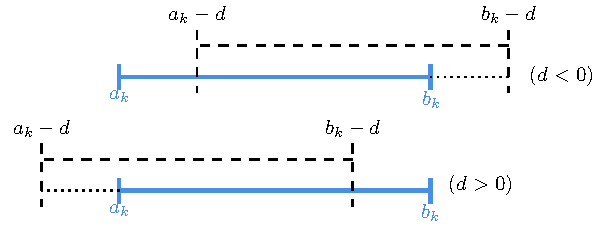
\includegraphics{figs14/1/fig1.pdf}
  \end{figure}
\end{frame}

\begin{frame}{Terminamos la Prueba}
  Entonces ocurre uno de los siguientes escenarios:
  \begin{itemize}
    \item $\tilde{E}\cup(\tilde{E}-d)\subseteq\bonj{a_k-|d|,b_k}$.
    \item $\tilde{E}\cup(\tilde{E}-d)\subseteq\bonj{a_k,b_k+|d|}$.
  \end{itemize}
  Estos intervalos tienen medida 
  \begin{align*}
    |d|+m(I)<\frac32m(I)&\To 2m(E) <\frac32m(I)\\ 
    &\iff m(E)<\frac34m(I)
  \end{align*}
  y esto nos lleva a una contradicci\'on.
\end{frame}

\begin{frame}{El Conjunto de Vitali}
  Definamos la relaci\'on de equivalencia sobre $\bR$:
  $$x\sim y\iff x-y\in\bQ.$$
  Llamemos $E_x$ a la clase de equivalencia de $x$, este conjunto es $\set{x+r:\ r\in\bQ}$. Note que $E_x$ es contable y por tanto hay una cantidad no contable de clases de equivalencia. El \alert{Conjunto de Vitali} es $E$, formado por un elemento de cada clase de equivalencia.
\end{frame}

\begin{frame}{Propiedades}
  \begin{itemize}
    \item $E$ es no contable.
    \item $(E-E)\cap U=\set{0}$.
  \end{itemize}
  Por el lema t\'ecnico \ref{lem:tecnicoVitali}, $E$ es no medible o bien $m_e(E)=0$. Pero como $\bR=\bigcup_{r\in\bQ}E+r$, entonces 
  $$m_e(E+r)=m_e(E)\neq 0.$$
  Concluimos que $E$ es no medible.
\end{frame}

\begin{frame}
  \begin{Cor}\label{cor:DeVitali}
    Sea $A\subseteq\bR$ con $m_e(A)>0$. Entonces existe $E\subseteq A$ tal que $E$ es no medible.
  \end{Cor}
  Como $\bR=\bigcup_{r\in\bQ}E+r$, entonces $A=\bigcup_{r\in\bQ}((E+r)\cap A)$. Llamemos $A_q=(E+q)\cap A$, un argumento similar al anterior muestra que $A_q$ es no medible.
\end{frame}
\section*{Resumen}

\subsection*{Qu\'e vimos hoy}

\begin{frame}{Resumen}

  % Keep the summary *very short*.
  \begin{itemize}
  \item El teorema \ref{th:caracMedibles} sobre una caracterización de conjuntos medibles con $G_\dl$'s y $F_\sg$'s. 
  \item El segundo teorema \ref{th:carac2Medib} sobre caracterizaciones.
  \item El teorema \ref{th:Caratheodory} de Carathe\'odory y un corolario \ref{cor:Caratheodory}.
  \item El teorema \ref{th:elTecnico} t\'ecnico.
  \item Aprendemos sobre el conjunto de Cantor \ref{ComienzaConjCantor}.
  \item El lema \ref{lem:tecnicoVitali} t\'ecnico usado para probar el resultado de Vitali. Y el corolario \ref{cor:DeVitali} que garantiza que hay m\'as de un conjunto no medible.
  \end{itemize}
  
\end{frame}

\subsection*{Ejercicios a trabajar}
\begin{frame}{Ejercicios}
    
  \begin{itemize}
    \item
      Lista 14
      \begin{itemize}
      \item La última parte de la prueba del teorema \ref{th:caracMedibles}.
      \item La prueba del teorema \ref{th:carac2Medib}
      \item Dos ejercicios \ref{ej:1baseTres} y \ref{ej:2baseTres} sobre base tres.
      \end{itemize}
    \end{itemize}
  
\end{frame}


% All of the following is optional and typically not needed. 
\appendix
\section<presentation>*{\appendixname}
\subsection<presentation>*{Lectura adicional}

\begin{frame}[allowframebreaks]
  \frametitle<presentation>{Lecturas adicionales}
    
  \begin{thebibliography}{10}
    
  \beamertemplatebookbibitems
  % Start with overview books.

  \bibitem{CambroNotas}
    S.Cambronero.
    \newblock {\em Notas MA0505}.
    \newblock 20XX.

    \bibitem{NachoNotas}
    I.Rojas
    \newblock {\em Notas MA0505}.
    \newblock 2018.
 
  \end{thebibliography}
  
\end{frame}
%% 6 - 2:10:52 48
%% 7 - 1:17:44 44
%% 8 - 27:37 69
%% 9 - 1:07:47 86 + 59:38 40 approx 2 h c 7 min
%% 10 - 2:22:39 63
%% 11 - Approx 2h c 2 min
%% 12 - Motiv y figs 1:00:17.53, en tot: 2:22:23.43
\end{document}


